\section*{Supplementary Material}
\subsection{Simulation Setting}
We generate response $Y_{ij}$ based on the following model

$$
Y_{ij} = \beta_0 + X_{ij} (\beta + \beta_i) + \V{Z}_{ij}\Tra ({b} + \V{b}_i) + \epsilon_{ij}, 
$$

where $\begin{cases} \beta_0 = 0.5 \\ \beta = 2 \\ b = 2 \\ X_{ij} \overset{i.i.d.}{\sim} Bernolli(0.5) \\ \beta_i \overset{i.i.d.}{\sim} Normal(0, 1) \\ \V{Z}_{ij}\Tra = (Z_{ij1}, Z_{ij2}, \cdots, Z_{ijK}) \overset{i.i.d.}{\sim} \mbox{MVN}(\V{0}, \M{I}) \\ Z_{ijk} \overset{i.i.d.}{\sim} Normal(0, 1) \\ \V{b}_i = (b_{1}, b_{2}, \cdots, b_{K})\Tra \overset{i.i.d.}{\sim} \mbox{MVN}(\V{0}, \tau^2\M{I})\\ b_{ik} \overset{i.i.d.}{\sim} Normal(0, \tau^2) \\ \epsilon_{ij} \overset{i.i.d.}{\sim} Normal(0, 1), i\in \{1,\dots,I\}, j\in  \{1,\dots,J\}\\ \end{cases}$.

 Note that $\beta_i$ is a scalar random effect and $\V{b}_i$ is a K-dimensional random effects. Testing $\V{b}_i$, that is, whether $\tau^2=0$ is of our interest. For both size test and power test, we have total sample size $I \in \{20,50,200\}$, and repeated visits $J \in \{20, 50\}$. According to the factorial design, we finally have six model designs $\{(I,J)\}\in \{(20,20),(20,50),(50,20),(50,50),(200,20),(200,50)\}$. Under each of the six model designs, dimension $K$ of the covariate $\V{Z}_{ij}\Tra$ varies in $\{2,4,8\}$. For test of size, we have data generated using $\tau^2=0$, and for test of power, we generate data using multiple different non-zero $\tau^2$ as $\{0.05^2, 0.07^2, 0.1^2, 0.15^2, 0.2^2\}$. Thus for test of size, considering different settings of sample size $I$, repeated visit $J$ and dimension $K$, for all of above $3\times 2\times 3=18$ model settings, we conduct the test $H_0$: $\tau^2= 0$ v.s. $H_a$: $\tau^2 > 0$ through 'exactRLR' based on 20000 times simulation; for test of power, with data generated using multiple different non-zero $\tau^2$, 3 different setting for sample size $I$, 2 different setting for repeated visit $J$ and 3 different settings for dimension $K$, and thus under each of above $18\times 5=90$ model settings, we conduct the test $H_0$: $\tau^2= 0$ v.s. $H_a$: $\tau^2 > 0$ through 'exactRLR' based on 20000 times simulation. For size test, simulated results showing around 5$\%$ type I error rate will be ideal, and for power test, as $\tau^2$ increases, an incremental power curve is expected. We use parallel computing to short the computation time.


\subsection{Simulation Results for Size Test}

\begin{table}[!h]
\caption{Table of size test under 18 model conditions by SVD decomposition transformation}
\centering
\begin{tabular}{c c c c c c c}
\toprule
%\toprule
{Model} & I=20,J=20 & I=20,I=50 & I=50,J=20 & I=50,J=50 &I=200,J=20 & I=200,J=50\\
\midrule
$K=2$ & 0.052 & 0.048 & 0.050 & 0.050 & 0.048 & 0.052 \\ 

$K=4$ & 0.050 & 0.050 & 0.050 & 0.049 & 0.051 & 0.049 \\ 

$K=8$ & 0.050 & 0.052 & 0.048 & 0.049 & 0.051 & 0.049\\ 

\bottomrule
\end{tabular}
\label{tab:sim_results for size test}
\end{table}
 Table 1 provides with the size test results based on 20000 times simulation under full combinations of the simulation design $I \in \{20,50,200\}, J \in \{20,50\}$, $K \in \{2,4,8\}$. As we can see, the test p-values fall in range $[0.048, 0.052]$, which demonstrate that our test procedure can well control type I error around 0.05, and maintain stable performance over change on sample size $I$, visit repeats $J$ and $K$.  
 
\newpage
\subsection{Simulation Results for Power Test}
\begin{figure}[h!]
\centering
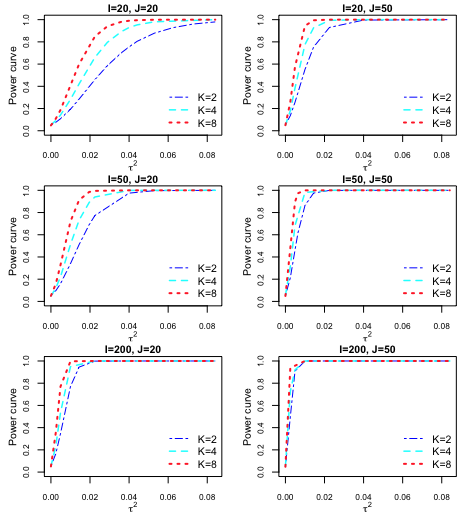
\includegraphics[width=0.9\textwidth]{power_suedo.png}
\caption{Power curve under different sample size $I$, repeated visit $J$, and $K$}
\label{power curve}
\end{figure}

Figure $\ref{power curve}$ illustrates the patten of power as the real variance $\tau^2$ increases from 0 up to $0.21^2$ under 18 different combinations of sample size $I$, repeated visit $J$, and $K$. Under all cases, a monotone increasing power curve with range from approximately 0.05 to 1 is observed. As one would expect, increase on the dimension $K$ of $\V{b}_i$ can lead to increasing test power when sample size $I$ and visit $J$ are fixed. As sample size $I$ increases, power of test will also increase and reach 1 much faster. Increasing visit $J$ can also increase test power. Actually the speed of test power converges to 1 is more sensitive to the affect of visit $J$ than sample size $I$, and thus power will reach 1 faster when $J$ is increased compared with $I$ is increased. For example, comparing the model condition $\{I=20, J=20, K=8\}$ with $\{I=20, J=50, K=8\}$ and $\{I=50, J=20, K=8\}$ respectively, we can see that power reaches over 0.9 at $\tau^2=0.1^2$ and is increased to about 1 at $\tau^2=0.12^2$ when $J$ is changed from 20 to 50 and $I$ stays 20, while power is around 0.7 at $\tau^2=0.1^2$ when $I$ is changed from 20 to 50 and $J$ stay 20. Similar situations can be observed in Figure $\ref{power curve}$.

